\frametitle{Phenytoin}
\begin{columns}
\begin{column}{0.6\linewidth}
	Phenytoin (C$_{15}$H$_{12}$N$_{2}$O$_{2}$, Dilantin) is a major antiepileptic drug (AED).
	Structure of phenytoin is a imidazolidine-2,4-dione that consists of hydantoin bearing two phenyl substituents at position 5, respectively.
	It is the most used drug for major epilepsy and the treatment of partial and generalised seizures such as tonic-clonic seizures.
	It also use as an antiarrhythmic, muscle relaxant, teratogenic agent, and a sodium channel promoter.
	Mechanism of action of Phenytoin acts by promoting sodium efflux from neurons in the motor cortex, reducing post-tetanic potentiation at synapses.
	The 3D structure of Phenytoin obtained from ZINC database with code 1665626.
%	Phenytoin is a well known inducer of CYP3A4 \cite{nishibe1995induction}.
\end{column}
\begin{column}{0.4\linewidth}
	\begin{figure}
		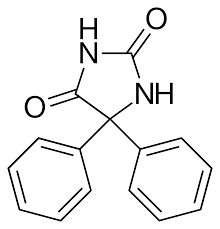
\includegraphics[width=0.8\linewidth]{phenytoin_str.png}
		\caption{\centering The structure of Phenytoin.}
		\label{fig:pht_str}
	\end{figure}
\end{column}
\end{columns}